\chapter{Quantitative dynamics of histones in the human cell nucleus}
\label{ch:frap}

  %% I decided to have a chapter precis. That is enough decorative
  %% test for the first page of a chapter.
%  \epigraph{Agora desenmerda-te.}{Portuguese ``saying''}

  %% chapter concept: in this chapter goes the whole kill FRAP project. I started
  %% positive that this should work and so should the text. We start by studying
  %% the technique and list the assumptions it requires. We do one experiment and
  %% face some problems. Each problem has its own section that ends in a solution.
  %% When the solution was not done, we could offer one. The last one is the cause
  %% that this is not possible and has no solution. Conclusion lists all problems
  %% and their solutions again.

  %% AF: Think this needs to be an abstract, summarising capter in 250 words
  %% Why would you have anything else than an abstract?

  \chapterprecis{
    To further the understanding of nucleosome structure and positioning
    in DNA, we aim to measure kinetic differences between wild type and
    mutant histones in live cells. Fluorescent Recovery After Photobleaching
    is a technique successfully used before to show the different kinetics and
    populations between different histone types. Using the same approach with
    our most disrupting histone mutant, we test the limits of FRAP when
    faced with extremely slow exchange ratios.
  }

  \section{Introduction}

  \subsection{Histone contribution to nucleosome dynamics}

    The building block of eukaryotic chromatin structure is the nucleosome, comprising
    \SI{147}{\bp} of DNA wrapped around an octamer of two copies of core histones H2A,
    H2B, H3, and H4 \citep{luger1997crystal}.
    Nucleosomes are arranged in a linear chain separated by DNA linkers, and
    can be further compacted into higher order chromatin structures.
    The role of chromatin not only encompasses DNA compaction,
    but also involves providing a dynamic complex to mediate access to genetic
    information by a capability to undergo reconfiguration of structure. \addref{Flaus?}

    Local reconfiguration of chromatin can be achieved
    by changing nucleosome structure or altering its composition.
    This can be performed through post-translational modifications
    or incorporation of histone variants,
    causing nucleosomes to alter DNA sequence preferences or recruit other proteins.
    Alternatively, chaperones and ATP-dependent chromatin remodelling complexes
    act extrinsically in nucleosome position.

    An important example of nucleosome remodelling is the SWI/SNF~complex
    whose deficiency causes growth defects in yeast.
    This complex was identified independently through screens for
    mating type SWIthching \citep{SWI-mutants}
    or Sucrose Non Fermentation \citep{SNF-mutants-original-discovery, SNF-mutants2}.

    A set of mutations have been uncovered that compensate
    for the loss of the SWI/SNF complex
    that are collectively known as SIN mutations because they
    provide SWI/SNF INdependence  \addref{?}.
    A subset of these are single amino-acid changes in core histones,
    providing a direct link between SWI/SNF and chromatin and suggesting
    that the histone mutation sites are involved in nucleosome dynamics and therefore
    of major importance in the nucleosome structure. This hypothesis has been tested \textit{in vitro}
    where SIN mutant nucleosomes display higher thermal mobility \citep{flaus2004sin}
    and observed in crystal structures of the mutants \addref{muthurajan2004crystal}.

    A complementary demostration of the effect of histone SIN mutants
    in the more complex \textit{in vivo} chromatin environment would
    validate the functional significance of these residues
    and contribute to the understanding of conservation of histone sequences

  \subsection{FRAP}

    Fluorescence Recovery After Photobleaching (FRAP) is an optical technique
    that reveals the dynamics of fluorescently tagged molecules within live cells.
    Tagged molecules inside a small region are irreversibly photobleached by
    action of a high-power focused laser beam and the recovery rate of fluorescence
    is measured. The recovery rate is interpreted as unbleached molecules
    from outside of the region at the time of photobleaching diffusing into the bleached area.
    It is assumed that this fluorescence recovery reflects natural protein movement.

    FRAP can be described by a simple chemical equilibrium:

    \begin{displaymath}
      F + S \overset{K_{on}}{\underset{K_{off}}{\rightleftharpoons}} FS
    \end{displaymath}

    where $F$ represents freely diffusing proteins, $S$ represents immobile vacant
    binding sites, and $FS$ the complex between the two, when the protein is bound
    to the binding site. This technique measures the value of \Kon{} and \Koff{},
    the association and dissociation constants by observing how fast a
    small population of photobleached $F$ in the $FS$ complex is replaced.

    This technique has been extensively used to obtain qualitative and quantitative
    insight on the kinetic properties of proteins, including histones \citep{KimuraCook}.
    These results show extremely slow recovery rates
    with histone residency half-lives longer than 8~hours.

    %% FIXME Much more descriptive on Kimura and Cook results

    Continuous development of FRAP has led to increasingly complex models
    that are both more precise and accurate than simple inverse exponential decay \addref{?}.
    Despite their sophistication, these models require certain important assumptions
    that are difficult to maintain for long experimental observation times:

    \begin{itemize}
      \item equilibrium is maintained throughout the entire experiment in
            order that both \Kon{} and \Koff{} remain constant,
            including that concentrations of both $F$ and $S$ remain constant;
      \item distribution of tagged molecule mimics the endogenous protein;
      \item the binding sites are part of a large, relatively immobile complex,
            on the time and length scale of the recovery.
    \end{itemize}

  \subsection{Aims}

    We wished to observe the structure--function relationship of the nucleosome
    using the histone SIN mutant H4~R45H that exhibited the
    highest increase in nucleosome mobility \textit{in vitro}.
    This led us to investigate the technical challenges of measuring subtle kinetic
    alterations of the nucleosome dynamics over long time periods in live cells.

  \section{Materials preparation}

%% This would need to be rewritten much more succinctly for a manuscript but is fine for thesis

  \subsection{Plasmid construction}

    Plasmids for the canonical histones H2B, H3, and H4,
    respectively pBOS--H2B--GFP \citep{KevinH2BGFP},
    pBOS--H3--EYFP.MC--N1, and pBOS--H4--ECFP.M--N1,
    were provided by Prof. Kevin Sullivan from National University of Ireland,
    Galway (NUIG). DNA sequencing identified the H3 plasmid as the HIST1H3B gene,
    encoding H3.1 from histone cluster 1; the H4 plasmid as either HIST1H4J or HIST1H4K;
    and the H2B plasmid similar to HIST1H2BJ but with missense mutations D25G and V118I.
    Plasmid pPAGFP--N1 and mCherry--\textalpha--tubulin were provided by Chelly van Vuuren
    and the HeLa cDNA library was a kind gift of Nadine Quinn \citep{NadineThesis}.
    Plasmid pMH3.2--614 including a mouse replication dependent histone~H3
    gene with upstream and downstream regulatory elements \citep{pMH3-plasmid},
    was provided by Prof. Kevin Sullivan.

    \paragraph{H2B--EGFP}
      The D25G and V118I mutations in pBOS--H2B--GFP were corrected by PCR mutagenesis
      using primers AFG114 and AFG115, and AFG112 and AFG113 respectively.
      The resulting product is H2B--EGFP, equivalent to the HIST1H2BJ gene product fusion.

    \paragraph{H4--ECFP R45H}
      The R45H mutation was applied to the pBOS--H4--ECFP.M--N1 by
      PCR mutagenesis using the primers AFG124 and AFG125. The codon
      \texttt{CAC} was selected for the histidine amino acid due to its
      higher codon usage in the human genome\citep{codon_usage}.

    \paragraph{H2A--EGFP}
      Plasmid pBOS--H2B--GFP was digested with KpnI and BamHI
      and the band corresponding to the linearised vector without the H2B sequence
      was purified by gel extraction. The HIST1H2AB sequence was amplified
      from HeLa genomic DNA with primers AFG116 and AFG118 and ligated into the vector.
      This coding sequence is equivalent to the H2A used in the previous
      \textit{in vitro} studies to be compared \citep{flaus2004sin}.
      HIST1H2AE has the same gene product but a lower codon adaptation index
      and more complex predicted 5' mRNA secondary structures.

    \paragraph{H2AX--EGFP and S139 mutants}
      Cloning of H2AX was similar to HIST1H2AB but used primers AFG130 and AFG131.
      Mutations to H2AX S139, an important site that is phosphorylated during
      DNA damage response, was performed at the same time of gene amplification
      since its location is close to the sequence 3' end. Primers AFG132, AFG133, and AFG134,
      were used with AFG130 to introduce mutations S139A, S139D, and S139E respectively.
      The mutation to alanine blocks, while mutation to aspartic and glutamic acid
      mimic phosphorylation. This strategy introduced an accidental frameshift mutation
      near the stop codon which was fixed by PCR mutagenesis using primers AFG400
      and AFG401.

    \paragraph{H2A.Z--EGFP}
      The H2A.Z sequence was amplified from an HeLa cDNA library
      using primers AFG121 and AFG122
      due to the existence of introns in the H2AFZ gene.
      Purification of the amplicon and ligation to the linearised pBOS--EGFP vector
      was identical to the preparation of the H2A--GFP plasmid.

    \paragraph{H4--EYFP}
      The plasmids pBOS--H3--EYFP.MC--N1 and pBOS--H4--ECFP.M--N1 were
      digested with the restriction enzymes BamHI and NotI. After agarose
      gel electrophoresis, the EYFP insert and pBOS--H4 vector were purified
      by gel extraction. The two DNA fragments were ligated to construct
      pBOS-H4-EYFP. The same strategy was used to construct the EYFP tagged
      H4~R45H mutant.

    \paragraph{H3--EYFP T45A and T45E}
      Mutations to H3 T45 were inserted into the pBOS--H3--EYFP.MC--N1 by
      PCR mutagenesis. The primers AFG151 and AFG152 were used for the
      T45E mutation, and AFG153 and AFG154 for T45A.

    \paragraph{H2B and H3 PAGFP}
      The PAGFP insert was prepared from pPAGFP--N1 by PCR using the
      primers AFG478 and AFG479, the amplicon purified by agarose gel
      extraction, digested with NotI and BamHI, and finally cleaned by
      PCR purification.
      Both pBOS--H2B--GFP and pBOS--H3--EYFP.MC--N1 plasmids were also
      digested with NotI and BamHI to excise their tags, and the vectors
      purified by agarose gel extraction. The insert was finally ligated
      into the two vectors for pBOS--H2B--PAGFP and pBOS--H3--PAGFP.
      This strategy introduces a Proline to Arginine mutation in the
      linker for the H2B plasmid.
      %% This mutation in the H2B linker (DPPVAT to DPRVAT) was on purpose.
      %% We could have easily avoid it but would cost us one extra primer
      %% and it shouldn't be making a difference.

    \paragraph{pMH2B--GFP and pMH3--EYFP}
      %% I'm actually not sure if Kevin gave me the pMH3.2--614 or the
      %% pCA-TAG plasmid. I did not have any plasmid map or sequence, only
      %% the very small Figure 5 of his paper PMID:9024683
      %% I couldn't even use any standard sequencing primer and by the time
      %% we cloned our genes there, we had already decided to kill the project
      %% so we never got to actually try these in human cells.
      Insertion of the H2B--GFP and H3--EYFP coding sequences into the
      pMH3.2--614 plasmid was performed by PCR amplification, bluent-end
      ligation of both vector and inserts due to the absence of restriction
      sites. pMH3.2--614 was amplified with primers AFG417 and AGF418 which
      create a linear sequence that only ignore the H3.2 coding sequence.
      The H2B--GFP coding sequence was generated with primers AFG419 and AFG420.
      Primers for the insert were phosphorylated by T4~PNK prior to the PCR
      since T4~PNK is more efficient on single stranded DNA. pM vector and
      H2B--GFP insert were purified by agarose gel extraction and ligated.
      Strategy for H3--EYFP was equivalent but using primers AFG424 and AFG420.

  \subsection{Cell lines}

    Transfection was always performed by lipofection~(\Sref{methods:lipofection}),
    both for transient and stable cell lines. For creation of stable cell lines,
    cells were trypsinized and split 1:20 on \SI{10}{\cm} dishes 24~hours after transfection.
    After another 24 hours, Blasticidin-S was added to the medium for
    a final concentration of \SI{3}{\ug\per\ml} as found by performing a
    Blasticidin-S kill-curve (\Sref{sec:methods:kill-curve}).
    Cell growth was followed and medium replaced when appropriate.
    As cell colonies started to be visible by the naked eye, approximately
    3~weeks after plating, these were screened by fluorescence microscopy.
    Positive colonies were aspirated and moved into 24-well plates with
    \SI{1}{\ml} disposable pipette tips, and the thinnest extremity removed.

    \begin{figure}
      \centering
      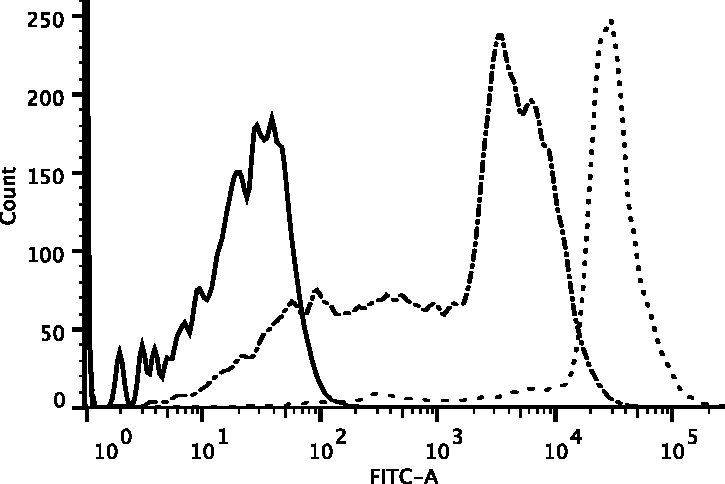
\includegraphics[width=\textwidth]{kill-frap/figs/facs-stable-cell-lines.pdf}
      \captionIntro{FACS sorting of mixed populations}
        {
          The multiple populations with differing intensity values were
          sorted by FACS. The full line represents the intensity profile
          of HeLa wild type cells; the dash-dot line, a mixed population
          of HeLa cells expressing H2B--EGFP; and the dotted line, the
          sorted population.
        }
      \label{fig:methods:facs}
    \end{figure}

    Populations with mixed levels of fluorescent intensity were frequently
    obtained while preparing stable cell lines. In such cases, cells with
    similar intensity of their corresponding fluorophore were FACS
    sorted (\fref{fig:methods:facs}).

    The following stable lines were prepared:

    \begin{itemize}
      \item HeLa H2B--EGFP
      \item HeLa H2B--EGFP D25G V118I
      \item HeLa H3--EYFP
      \item HeLa H3--EYFP T45A
      \item HeLa H3--EYFP T45E
      \item HeLa H4--EYFP
      \item HeLa H4--EYFP R45H
    \end{itemize}

  \subsection{Microscopy}

    Both stable and transiently cell lines were used in imaging as described.
    Transfection was performed 48~hours before imaging for transiently
    expressing cells.

    Confocal microscopy was performed with a Zeiss LSM510 Meta microscope
    using glass bottom LabTek II chambers. Wide-field fluorescence microscopy
    was performed with an Applied Precision DeltaVision Core system
    using \SI{35}{\mm} glass bottom MatTek dishes.

    In both cases, imaging was performed within an acrylic environmental
    chamber that fully enclosed the stage plate and microscope objectives.
    Temperature and CO$_2$ levels were maintained via separate units connected
    to the environmental chamber.

  \subsection{Computational analysis}

    Software used for image analysis and visualization was described in
    \Sref{sec:methods:software}. Original source code written in \textsc{Matlab} for a previously
    reported circle FRAP model \citep{mueller2008evidence} was kindly offered
    to us under the GNU General Public License (GPL) version~3 by the
    original authors. A port of this code for the GNU Octave language was
    prepared and made available under the same license.

  \section{Results}

  \subsection{FRAP analysis in Octave}

    In order to estimate binding constants from FRAP data, we ported
    \textsc{Matlab} code for circle FRAP \citep{mueller2008evidence} to GNU Octave.

    Functions for nonlinear regression were required for the model
    fitting and were replaced by \texttt{leasqr}
    from Octave-Forge's optim package. This function performs the
    Levenberg--Marquardt nonlinear least squares algorithm which is the
    same as the documented method for \texttt{nlinfit}.
    Several sample images were analyzed
    by the Octave port and the fitted values were found to be equal to
    the values reported by the authors using the original code (data not shown).
    Functions for graphical user interaction were mainly required
    for manual selection of Regions Of Interest (ROIs) and options.
    Selection of ROIs was replaced by automatic identifications
    and parameter input was made command-line based for batch processing.

    \subsubsection{ROI selection}

      Bleach spot, nucleus region, and background region ROIs are required
      for the circle FRAP model. The bleach spot measures intensity recovery
      and also models the photobleach profile since it takes into account
      a non-uniform spatial distribution of the bleached spot. The nucleus
      region defines the finite sized nucleus and takes into account
      the fluorescence loss during the photobleaching,
      while a small region outside the nucleus is used for background correction.

      Cells expressing GFP tagged histone proteins have well defined nuclei.
      The large amount of histone protein and specificity for nuclear chromatin
      produces a strong and clear signal for the nuclei contrasted on a dark background (\fref{fig:kill-frap:roi}).

      \begin{figure}
        \centering
        \subbottom[pre-bleach]{
          \includegraphics[width=0.45\textwidth]
          {kill-frap/results/roi-prebleach.png}
          \label{fig:kill-frap:prebleach}
        }
        \hfill
        \subbottom[post-bleach]{
          \includegraphics[width=0.45\textwidth]
          {kill-frap/results/roi-postbleach.png}
          \label{fig:kill-frap:postbleach}
        }
        \subbottom[pre-bleach $-$ post-bleach]{
          \includegraphics[width=0.45\textwidth]
          {kill-frap/results/roi-subtracted.png}
          \label{fig:kill-frap:subtracted}
        }
        \hfill
        \subbottom[Identified ROIs]{
          \includegraphics[width=0.45\textwidth]
          {kill-frap/results/roi-selected.png}
          \label{fig:kill-frap:selected}
        }
        \captionIntro{Automatic selection of ROIs for FRAP}
          {
            HeLa stable cell line expressing the H4~R45H mutant tagged with YFP,
            are imaged every \SI{30}{\ms} in a confocal microscope. A circular
            shape is used for photobleaching after 100~frames.
            \subcaptionref{fig:kill-frap:prebleach} averaging of 50~pre-bleach
            images removes most of the noise, allowing for a better refined
            ROI;
            \subcaptionref{fig:kill-frap:postbleach} average of
            5 post-bleach images;
            \subcaptionref{fig:kill-frap:subtracted} subtraction of the
            post-bleach to the pre-bleach image, gives a clear indication
            of the bleach spot, as well as faint signal for the nuclear
            region due to unintentional photobleaching;
            \subcaptionref{fig:kill-frap:prebleach} perimeter of the
            automatically identified ROIs superimposed on the pre-bleach
            image: cell nuclei, bleach spot, and background region.
          }
        \label{fig:kill-frap:roi}
      \end{figure}

      Subtraction of the post-bleach (\fref{fig:kill-frap:postbleach}) from
      the pre-bleach (\fref{fig:kill-frap:prebleach}) images displays
      a clear circular shape corresponding to the bleach spot (\fref{fig:kill-frap:subtracted}).
      The centre for this spot was identified by finding the maximum of the convolution matrix
      between the subtracted image and a disk kernel.
      To reduce signal-to-noise ratios, multiple pre and post-bleach images of the cell
      were averaged before image operations.
      While the bleach spot is the most visible feature, there is a faint nuclear region signal
      caused by background photobleaching during image collection.

      An approximate border for cell nuclei could be readily defined using Otsu's method for image threshold.
      As with the identification of bleach spots, multiple pre-bleach images
      were averaged before threshold definition for a more accurate cell border (\fref{fig:kill-frap:selected}).
      Since multiple nuclei often appeared in a single image, the coordinates for the bleach spot
      were used as reference to select the correct nucleus.
      The background region was identified by finding the minimum of the convolution matrix
      between the averaged pre-bleach images and a small square of black intensity values.

    \subsubsection{Batch processing}

      \begin{sidewaysfigure}
        \includegraphics[width=\textwidth]{kill-frap/results/frapinator.png}
        \captionIntro{Frapinator visual log files for batch processing}
          {
            Each FRAP experiment generates a log file with 6 different plots
            displaying the analysed values and the fitting to different models.
            In conjunction with the images in \fref{fig:kill-frap:roi} this
            provides a quick overview of the entire analysis process.
            The top left plot displays the raw intensity
            for the background, bleach spot, and nucleus intensity over the
            duration of the FRAP experiment. This is followed by the normalized
            intensity for the bleach spot which is actually used for the
            fitting. The top right displays the intensity
            profile for the bleach spot, and its fit to a radial profile
            model. The three bottom panels display the data fitted to three
            different models: pure diffusion which has no terms for binding
            constants; full model with a fixed diffusion rate; and full model
            with all the 3 terms.
          }
        \label{fig:kill-frap:frapinator}
      \end{sidewaysfigure}

      The automated identification of ROIs was turned into a stand-alone program, frapinator.
      This has the advanatge that the user can set command-line options without scripting.
      Representative images are saved with results and all intermediate analysis is logged for post-processing analysis.
      These include the automatically identified ROIs and
      plots of measured intensities, bleach spot profile, and fitting to different models \fref{fig:kill-frap:frapinator}.
      Frapinator is available for public download under the GPL \footnote{\url{https://github.com/af-lab/frapinator}}.

  \subsection{Tracking of cell nuclei}

    %% We could show this but it would only be to "encher chouricos"
%    \begin{figure}
%      \centering
%      \missingfigure{Our first FRAP experiment}
%      \captionIntro{Long time series of HeLa cells expressing H2B--EGFP.}
%                   {Cells were transfected with pBOS--H2B-EGFP and imaged for 8
%                    hours, with intervals of 20 minutes.}
%      \label{fig:kill-frap:cell-movement}
%    \end{figure}

    Histone proteins exhibit extremely slow kinetics of exchange
    requiring FRAP to be performed over several hours during which cell movement is
    a particular issue. % \fref{fig:kill-frap:cell-movement}.

    %% This needs some sentences describing the nature of effects of the movement,
    %% and a semi-emirical statement of the scale of the movement
    %% since this problem is the nub of the entire chapter.
    %% Need to justify the need for going to the trouble
    %% and define threshold for success (that couldn't be achieved!)

    The central requirement to accurately identify and quantitate the signal
    in the photobleached spot led us to pursue both cell biological approaches to
    minimise cell movement and and computational approaches to track imaged regions.

    \subsubsection{Contact inhibition at high cell density}

      Mammalian cells display contact inhibition,
      a cellular growth mechanism by which cells enter senescence and reduce motion
      when surrounded by other cells with no free space for movement.
      Although transformed cell lines lose this property,
      reduced space does place a restriction in the movement.
      %% Can you provide a semi-quantitative estimate of the cell density you mean?
      We attempted to use this effect to limit movement of cells
      by performing FRAP measurements with cells at higher confluence levels.
      We observed some decrease of movement for HeLa cells but not a complete immobilization.
      %% Can you provide a semi-quantitative estimate of the degree of reduction in movement?

      \begin{figure}
        %% We are only showing one cell rather than the whole field of
        %% of view because otherwise it's hard to notice the movement of
        %% individual cells. If we do display everything, we cell many
        %% nuclei that seem like their movement is smaller. If we do
        %% show it, we comment that we are unsure whether the movement
        %% is cellular or only nuclear.
        \centering
        \includegraphics[width=\textwidth]{kill-frap/results/confluent-hela.png}
        \captionIntro{Movement of confluent HeLa cells during FRAP experiment}
          {
            Cells reached confluence before the start of the
            experiment in an attempt to reduce motion. Instead, this caused
            cell nuclei to undergo heavy reshape as the cell apparently
            squeezes in between its neighbours. Half-nuclear FRAP performed in
            a confocal microscope over an interval of 8~hours. Top left panel
            is the pre-bleach image, while the others have a time-interval of
            21~minutes. Cells are a stable line derived from HeLa, expressing
            the H4~R45H mutant tagged with YFP.
          }
        \label{fig:kill-frap:confluent-hela}
      \end{figure}

      Tracking of the ROIs over time was still required \fref{fig:kill-frap:confluent-hela}.
      %% Isn't this out of order since CropReg section is below.
      %% Even if you did it in a different order, why not put the horse cells first.

    \subsubsection{Primary cell lines}

      Since HeLa cells have lost the ability to activate contact inhibition,
      we obtained an immortalised primary horse fibroblast cell line
      that displayed contact inhibition. Using this cell line we could
      maintain a layer of healthy cells covering a Petri dish for several days???
      after reaching confluence (data not shown).
      %% Cell growth was halted instead of becoming over-confluent ???what do you mean???
      %% Although obvious, it would be good to have some sort of image to justify the statement?

      However, primary cell line transfections have typically much lower efficiency rate and
      confluent cells have lower expression with each cell division.
      To balance transfection efficiency and expression we transfected cells at
      \SI{70}{\percent} confluence and imaged them after 3 days.

      Even after reaching confluence, we observed movement of transfected horse cells \fref{fig:kill-frap:confluent-horse}.
      %% Is there some sort of relative statement about the degree of reduction or residual movement?
      In addition, the observed movement was dramatically different in primary horse than in HeLa cells.
      Transfected horse cells displayed a helical motion about the vector of their movement
      whereas rotation of HeLa nuclei was mostly restricted to the $z$ axis.
      %% You need to define the coordinate system to talk about z axis!
      %% Do you mean vertical relative to the cell dish layer?

      \begin{figure}
        \centering
        \includegraphics[width=\textwidth]{kill-frap/results/confluent-horse.png}
        \captionIntro{Movement of confluent primary cells during FRAP experiment}
          {
            Primary horse fibrolasts display contact inhibition and halt growth
            once they reach confluence. However, this does not stop cell
            motion which can still be seen moving. In addition, when compared
            to the cancer cell line HeLa (\fref{fig:kill-frap:confluent-hela}),
            the horse fibroblasts frequently rotated around the $x$ and $y$
            axis. Circle FRAP was performed in a widefield microscope.
            Top left panel is the pre-bleach image, while the others have a
            time-interval of 15~minutes. Cells were transiently transfected
            and are expressing H2B type1-J tagged with EGFP.
          }
        \label{fig:kill-frap:confluent-horse}
      \end{figure}

    \subsubsection{Tracking of cell movement}

      As an alternative strategy, we implemented cell tracking
      in order to transform images into a common frame using
      consecutive image cropping and image registration.
      This approach was implemented as a program named CropReg.

      Nuclei of interest were tracked by template-based matching using normalized cross-correlation.
      Briefly, the nucleus to track was identified on the first frame and
      used as template against the image on the subsequent frame.
      For increased performance and robustness only the region surrounding the original position is used.
      %% Should you state approximately how large this region was?
      Sequentially applying this method created a stack of smaller images centred on the nuclei of interest.

      Achieving this functionality required implementing a ``coeff'' option
      for scaling in the \texttt{xcorr2} function in GNU Octave.
      This was contributed and released in version 1.2.0 of the Octave Forge signal package.
      %% TODO since there's more than one way to actually do the normalization,
      %% it might be a good idea to write down the actual math formula
      To correct for rotational movement around the $z$ axis,
      frames were aligned using rigid body geometric transformation using ImageJ plugin StackReg \citep{stackreg}.

      \begin{figure}
        \centering
        \includegraphics[width=\textwidth]{kill-frap/results/cropreg.png}
        %% imaging was done every 10 minutes, but we are skipping
        %% every other panel
        \captionIntro{Automatic tracking and alignment of moving cells}
          {
            Using CropReg, we successfully tracked individual cells during
            a time-series microscope experiment. The top left corner of each
            panel displays the tracked and aligned cell. Imaging was performed
            in a widefield microscope. Time interval between panels 20~minutes.
            Cells are a stable line derived from HeLa, expressing H3 tagged
            with YFP.
          }
        \label{fig:kill-frap:cropreg}
      \end{figure}

      Using this image processing approach we were able to track individual cell nuclei
      throughout an entire sequence of FRAP experiments \fref{fig:kill-frap:cropreg} provided
      that nuclei did not overlap.
      Although only a small minority of image sequences satisfied this requirement,
      it was possible to collect sufficient observations for FRAP calcultions.

  \subsection{Chromatin movement}

    While performing the FRAP experiments, we observed some movement
    within the cell nuclei. These could not be accounted for simple rotational
    movement around the $x$ or $y$ axis, and resembled more the movement
    of individual bodies within the nuclei.

    \subsubsection{Selection of \G1{} cells}
      %% There's no chemical equilibrium in S phase

      A possible cause of this chromatin movement comes from changes in
      the cell cycle phase. During the S~phase, the DNA is replicated,
      doubling the content of the chromatin.
      More importantly, this breaks
      a core assumption of FRAP, that the system remains in equilibrium
      during the entire experiment. This does not hold if the DNA, the
      binding sites for our model, duplicate in number.

      If the FRAP experiments can't be performed during S~phase and
      mitosis, we are limited to \G1{} and \G2{}. Considering
      the length of the HeLa cell cycle and the requirements to image
      for a time period of 8~hours, we are further limited to \G1{}.
      In addition, the FRAP experiment must be performed early in
      \G1{}~phase to avoid crossing over to the S~phase.

      %% The only reason this was required was because the LSM 510
      %% that we were using could not make Z stack and time lapse
      %% at the same time.
%      \begin{figure}
%        \centering
%        \missingfigure{Hela cells splitting}
%        \captionIntro{Picking cells at early G$_1$.}
%                     {We imaged cells that were entering mitosis and picked their
%                      daughter cells for the FRAP experiments. Because HeLa cells lift
%                      away from the dish during mitosis, opening the
%                      pinhole and set the Z-center in between the cell dividing plane
%                      and dish bottom was necessary. Ends up nothing being properly in focus but we
%                      can track things fine. Of course, some cells still floated away.}
%        %% TODO explicit parameters
%        \label{fig:kill-frap:picking-early-g1}
%      \end{figure}

      To do this, cells in mitosis were selected and tracked during 4~hours.
      After this time period, we used the daughter cells which we could be
      confident of being in early \G1{}.
      %% we also waited some 2 hours after mitosis since that's when cells
      %% unpack their chromosomes.

      During mitosis, HeLa cells form a sphere slightly above the plane of
      other cells, and keep a weak connection to the growth surface.
      Because of this, they easily detach, which is the basis for the
      mitotic shake-off method, and float away from the field of vision
      which requires a larger number
      of initial selected cells. In addition, to minimize any effect that
      may arise from imaging, it was done at minimal laser power and every
      30~minutes, just enough to allow manual tracking.
      Finally, since our system did not permit simultaneous Z-stack and time
      lapse imaging, and cells in mitosis are in a separate focal plane,
      imaging was performed with the pinhole sized to the max and focused
      in between the two planes. While this
      created very blurred images, it allowed to visualize all cells during
      the entire procedure.

      However, even after selecting cells in this cell cycle, movement within
      the bleach spot could still be observed.

    \subsubsection{Inverse FRAP}

      Due to the non-homogeneous nature of the chromatin, it was difficult
      to assess the total extent of the observed movement. To
      better visualize this, we performed inverse FRAP which allows us
      to track the movement of the bleach spot only.

      For this purpose, we replaced the EGFP tag in our H2B plasmid
      with photoactivatable GFP (PAGFP), a GFP derivative that requires
      activation by a specific wavelength to become fluorescent. This
      allows us to activate a specific spot of the nucleus and visualize
      its movement.

      Since PAGFP cannot be easily detected before photoactivation, cells
      were co-transfected with mCherry--\textalpha--tubulin which localises
      exclusively to the cytoplasm, giving an outline of the nuclear region
      \fref{fig:kill-frap:ifrap}.

      \begin{figure}
        \centering
        \subbottom[pre-activation]{
          \includegraphics[width=0.45\textwidth]
          {kill-frap/results/ifrap-pre.png}
          \label{fig:kill-frap:ifrap-pre}
        }
        \hfill
        \subbottom[post-activation]{
          \includegraphics[width=0.45\textwidth]
          {kill-frap/results/ifrap-post.png}
          \label{fig:kill-frap:ifrap-post}
        }
        \subbottom[activated spot over time]{
          \includegraphics[width=\textwidth]
          {kill-frap/results/ifrap.png}
          \label{fig:kill-frap:ifrap-timeframe}
        }
        \captionIntro{Inverse FRAP experiment showing chromatin movement}
          {
            HeLa cells co-transfected with mCherry--\textalpha--tubulin and
            H2B type1-J tagged with PAGFP.
            \subcaptionref{fig:kill-frap:ifrap-pre} The cell nucleus, target
            for photoactivation, can be easily identified as the ``empty''
            region via the mCherry channel on which would otherwise be an
            invisible feature on the GFP channel;
            \subcaptionref{fig:kill-frap:ifrap-post} spot after activation;
            \subcaptionref{fig:kill-frap:ifrap-timeframe} detail of the
            activated spot every 20~minutes. Rather than a gradual loss of
            fluorescence that maintains the circular shape, the activated spot
            kind of unfolds itself spreading the region of interest.
          }
        \label{fig:kill-frap:ifrap}
      \end{figure}

      Using this FRAP variant, the movement of chromatin was more noticeable.
      Rather than an homogeneous loss of fluorescence, the activated
      spot uncurled itself overtime with individual branches of
      localized PA-GFP appearing in the nuclei (\fref{fig:kill-frap:ifrap}).

  \section{Discussion}

  Performing FRAP of histones requires an extension of the experiment over
  its typical length. \cite{KimuraCook}
  reported that the recovery was not complete, even after 8~hours.
  We aimed at compare kinetic constants of wild type histones against
  specific mutants, and used a previously reported model for circle FRAP
  which had already been validated against other fluorescent techniques,
  and reported to account for multiple errors in a typical FRAP modelling.

  However, simply collecting valid recovery data for such a long time
  period is an issue on its own.

  \subsection{Cell movement}

    The first problem to expect when performing such experiment over
    long times is cell movement. This is a natural occurrence and cells
    where movement is absent are likely to be dead. But as the nuclei
    movement is mostly translational and rotational around the $z$ axis,
    a single spot can still be tracked in a single focal plane.

    \label{sec:kill-frap:discuss-contact-inhibition}

    We attempted to eliminate cell motion by inducing contact inhibition,
    a feature of normal cells to control cellular growth. As cells reach
    higher densities, they move into the \G0{}~phase of the cell cycle,
    entering a quiescent state. In tissue culture,
    this translates to a stop in proliferation, and formation of a monolayer
    of healthy cells in the flask. This requires the use of primary
    cell lines since these have not lost this feature yet.

    This is a very attractive strategy for reducing motion due to the
    fact that this is a natural occurring mechanism. Nonetheless,
    other factors must be taken into consideration.
    Increased difficult on cell handling, and reduced
    transfection efficiency are only labour related, but it also means
    that stable cell line cannot be used. Most importantly, immortalized
    cell lines such as HeLa are standard in cell biology which makes
    comparisons to other studies much more conclusive.

    However, while we did observe a monolayer of healthy cells develop,
    and maintained stable over 2 weeks, observation of individual transfected
    cells still showed movement. In addition, the nature of the movement
    had changed and instead of the simple translational movement observed
    in the HeLa cells, all nuclei displayed an helix-like movement on the
    direction of the movement (\fref{fig:kill-frap:confluent-horse}).

    %% Meth! Not even once.
    The possibility of using drugs to reduce motion was also briefly
    considered. Previous FRAP of histones was performed using
    multiple inhibitors of protein synthesis, which reported different
    histone kinetics for the same histones \citep{KimuraCook}. Their
    conclusion was that the results were ``difficult to interpret''.

    Ultimately, we solved this problem by writing our own program
    for cell tracking by normalized cross-correlation template matching, a
    well-known technique. Not only was this technique sufficient for our
    case, it also avoided the usage of any drugs that could affect the
    conclusions and add another variable.


  \subsection{System equilibrium}

    The basis behind a FRAP experiment is a chemical equilibrium on
    formation of a complex between the freely diffusing proteins and
    vacant binding sites, and for the equilibrium to be maintained,
    concentrations of both reactants must remain constant.
    When the system is the intra cellular environment, achieving
    true chemical equilibrium is inconceivable but for the purpose
    of a FRAP experiment, certain efforts can be taken to reach a
    compromise.

    In our specific case of FRAP for histone
    dynamics in chromatin, the equilibrium is between
    a soluble pool of histone proteins, and formation of a nucleosome
    bound to the DNA. This translates in a requirement to maintain the
    amount of proteins and DNA constant. If FRAP was performed in the
    time-scale of seconds or even minutes,

    \subsubsection{DNA replication}

      %% Interesting: the paper "A search for differential polypeptide synthesis
      %% throughout the cell cycle of hela cells", on Journal Cell Biology 1980,
      %% vol 84 795-802 by Rodrigo Bravo and Julio E. Celis, says about HeLa
      %% cell cycle on page 796 that "average duration of G1, was 11.7 h; S was
      %% 8.8 h; and G2 and M was 4 h. The division time was 24.5 h." However,
      %% the technique they refer mention much shorted times.
      %% They reference "Growth and nucleic acid synthesis in synchronously
      %% dividing populations of HeLa cells", on Experimental Cell Research
      %% 1963, vol 30 344-362 by T. Terasima and L.J. Tolmach which on Table III
      %% in page 354 have a median doubling time of 21h (which is actually quite
      %% shorter than the typically reported 24h for HeLa under optimal
      %% conditions), and 8.5h for G1, 9.5h for S, 2.3 for G2, and 0.7h for M.
      %% So HeLa cells from the 60s are different from the cells of nowadays?

      \begin{figure}
        \centering
        %% based on original code from Robert Vollmert
        %% http://www.texample.net/tikz/examples/pie-chart/
        \newcommand{\slice}[4]{
          \pgfmathparse{0.5*#1+0.5*#2}
          \let\midangle\pgfmathresult

          % slice
          \draw[thick,fill=black!10] (0,0) -- (#1:1) arc (#1:#2:1) -- cycle;

          % outer label
          \node[label=\midangle:#4] at (\midangle:1) {};

          % inner label
          \pgfmathparse{min((#2-#1-10)/110*(-0.3),0)}
          \let\temp\pgfmathresult
          \pgfmathparse{max(\temp,-0.5) + 0.8}
          \let\innerpos\pgfmathresult
          \node at (\midangle:\innerpos) {#3};
        }
        \begin{tikzpicture}[scale=3]
          \newcounter{a}
          \newcounter{b}
          %% Total cell cycle is 24.5 hours, G1 is 11.7h, S is 8.8h,
          %% G2 is 3h, M is 1h. The problem is that the counters can't handle
          %% decimal places so we have a variable with the actual time for
          %% the text, and another one times 10 to calculate the angle.
          \foreach \p/\t/\l in {117/11.7/\G1, 9/0.9/M,
                                31/3.1/\G2, 88/8.8/S}
            {
              \setcounter{a}{\value{b}}
              \addtocounter{b}{\p}
              \slice{36*\thea/24.5} % we multiply by 36 instead of 360 because
                    {36*\theb/24.5} % the time is already times 10
                    {\l}{\t{} hours}
            }
        \end{tikzpicture}
        \captionIntro{HeLa cell cycle phases and choice of timing}
          {
            Under optimal growth conditions, the HeLa cell has a median
            doubling time of approximately 24.5~hours, with \G1~and
            S~phases alone having a length of 11.7 and 8.8 hours each \citep{HeLaCellCycle}.
            Since the FRAP experiment must avoid the S phase and last for
            at least 8~hours, the only possibility while using cells in normal
            growth conditions is to start the experiment in the early \G1~phase.
          }
        \label{fig:kill-frap:cell-cycle}
      \end{figure}

      %% How we got to 3.1 hours for G2 phase: in 1980, they reported 4h
      %% for G2 and M phases together. In 1963 they specified 2.3 and 0.7
      %% for each, so the total increased by 1/3 (from 3 to 4 hours).
      %% I'm assuming 2.3 + 2.3*1/3

      DNA replication happens during the S~phase which breaks the equilibrium.
      In addition, the entire replication machinery will move through the DNA
      strands, displacing nucleosomes. This limits the experiment from the
      interphase to either \G1{} or \G2{} phases. However, considering
      the HeLa cell cycle has an average \G2{} phase of 3~hours, and even
      \G1{} is 11.7~hours long \citep{HeLaCellCycle}, the FRAP experiment
      becomes limited to a start on early \G1{} (\fref{fig:kill-frap:cell-cycle}).

      %% papers from Andrew Belmont. Search finite time potential 'spatial disequilibrium'

      %% When I was at Jim McNally's lab, Timothy Stasevich was leaving to
      %% work on Hiroshi Kimura's lab and heard that he had found some
      %% fancy dynamics for DNA binding proteins on the early 3 hours of G1.
      %% It was not published back then, and I couldn't find it.
      In addition, post-mitotic chromosomes take some time to rebuild the
      interphase nuclear architecture during early \G1{}. After decondensation,
      chromosome territories move within the nuclei to similar neighbourhoods
      as their mother nucleus, a process that has been estimated to
      take approximately 2 hours
      \citep{visualizationG1chromosomes,earlyg1position,RelativeChromosomePosition}.
      This further limits the timing to start a FRAP experiment to a very
      small window.

      We solved this problem in a rather ingenious method, minimizing
      intervention on the cell normal growth. We tracked cells manually during
      mitosis where visual identification of the cell cycle is possible,
      therefore limiting the experiment to individual cells exactly 3 hours
      after start of \G1{}.
      Its only drawback is extending the total imaging time which
      requires a microscope chamber with a controlled environment.
      However, this problem only arises because the FRAP experiment itself
      is long enough to already require such chamber. Furthermore, since these
      images are only meant for manual tracking of cells and have no
      quantitative purpose, time interval between images can be increased,
      the both resolution and laser intensity reduce to the minimum, to
      minimize any phototoxicity arising from the extra imaging.

      %% Present many methods to control cell cycle
      %% Basically, we already solved the problem with a program and
      %% picking the right cells. These are just other things we considered
      %% but none is as clean as our solution.

      This whole problem can be reduced to an issue of cell cycle control and
      several other options were considered which may be of interest for
      other FRAP experiments. The most common solution is the use
      of drugs for cell cycle arrest, an option that has already been
      discarded since, as previously discussed for cell movement, has been
      shown to have to great of influence in the results.
      In addition, since arrest on \G1{} is only
      performed at its interface to S~phase, cells would be under their
      effect for the duration of an entire cell cycle as well as the FRAP
      experiment.
      Serum starvation is a frequently used ``natural''
      alternative to move cells from the normal cell cycle into the
      quiescent \G0{} phase \citep{SerumStarvation}.
      Primary cells that divert naturally into \G0{} as part of
      the contact inhibition response, were also considered but
      discarded as already discussed on \Sref{sec:kill-frap:discuss-contact-inhibition}.

      For cases where even longer times could be required, there are cells
      with longer cell cycles. Pancreatic cancer cell lines are well-known
      for displaying a specially slow growth, with Capan-1 among the slowest
      and displaying a median doubling time of 60~hours \citep{PancreaticCells}.

    \subsubsection{Protein expression}

      The other reactant is the tagged histone protein which is being
      constitutively expressed under control of the EF-1\textalpha{} promoter,
      part of the pEF-BOS vector. This can be a problem not only because it
      disturbs the equilibrium, but also because it differs from the endogenous
      histone expression ultimately leading to a different distribution in the
      chromatin \citep{KimuraCook}.
      While the first issue can be resolved with the use of protein synthesis
      inhibitors, and indeed \cite{KimuraCook} used cycloheximide (CHX) and
      5,6-Dichloro-1-\textbeta{}-D-ribofuranosylbenzimidazole (DRB) for this purpose,
      this does not address the second issue.

      %% TODO: would be cool to create this figure
%      \begin{figure}
%        \centering
%        \missingfigure{a schematic of cell cycle, soluble pool}
%        \captionIntro{Distribution of tagged and endogenous histones during cell cycle}
%                     {
%                       This would be at least 3 different subplots. The first
%                       and the second are like the ones in Fig 7A of Kimura and
%                       Cook paper. The third one would show the ratio of each
%                       histone over time, i.e., 100\% tagged during all cell
%                       cell cycle and some endogenous during S phase. In this
%                       plots, also note where euchromatin and heterochromatin
%                       are replicated.
%                     }.
%        \label{fig:kill-frap:messy-histone-expression}
%      \end{figure}

      The histone expression profile is highly regulated
      for expression during the S~phase, when it suffers a 35-fold
      up-regulation. This is likely to be related with the high
      demand of histones to package the newly duplicated genome.
      Histone proteins in a soluble pool are incorporated into the
      genome as this is duplicated, but because the tagged histones are
      expressed during the entire cell cycle, the ratio between tagged and
      endogenous histones varies through the S~phase, being higher in the
      early S~phase when expression of the endogenous histone has just started.
%      (\fref{fig:kill-frap:messy-histone-expression})
      If there is an higher
      ratio of tagged histones in early S~phase, and since genome regions with
      higher transcriptional potential are replicated earlier in this phase
      \citep{DNA-replication-timing}, tagged histones will be incorporated
      preferably in this regions where they will naturally display higher kinetics
      rates. Their global distribution in the genome will not
      mimic the endogenous protein \citep{KimuraCook}, a basic assumption of
      the FRAP experiment.

      Another view is that histone expression is not up-regulated in
      S~phase, but rather down-regulated for the rest of the cell cycle.
      Histone proteins have an high affinity to DNA and in excess
      can block access to it, leading to multiple defects in unicellular
      organisms, but also in animal development including lethality in \species{Drosophila}
      \citep{excess-histone, regulated-histone-proteolysis, drosophila-excess-histone1,
      drosophila-excess-histone2}.

      Histone transcript regulation is a well studied mechanism,
      and mostly performed by histone specific 3' UTR elements,
      a stem-loop and a purine-rich Histone Downstream Element (HDE) that
      replace the typical poly(A) tail. These elements maintain stability
      of histone mRNA during S~phase only, but are absent from the
      pBOS vector and tagged histones are translated with a poly(A) instead.
      An expression vector that mimics the endogenous histone regulation
      would be the perfect solution. Expression limited to S~phase would
      stop expression during \G1{}, the cell cycle phase to which we are
      already constrained, maintaining the required chemical equilibrium.
      It would mimic the chromatin distribution of the endogenous histones,
      prevent any effects that arise from excess of histone proteins, and
      avoid usage of biosynthesis inhibitors. Finally, the time interval
      between end of expression and FRAP, between S~and \G1{}, even allows
      for GFP to fully mature and become fluorescent.

      Such vector has been already prepared by cloning an entire replication
      dependent histone~H3 gene, including the upstream and downstream
      regulatory elements \citep{pMH3-plasmid}. As this system is unique to
      replication dependent histones, it is a valid question whether it
      would handle different proteins, even a GFP tagged histone, but
      this has already been done. The H3 coding sequence of the mentioned
      plasmid has been replaced with a CENP--A tagged on its C--terminus with
      HA1 for exactly the same purpose, restrict expression of the
      tagged protein to the S~phase \citep{Kevin-pCA-TAG}.

      The only difficulty this can pose is on cloning, due to the lack of natural
      restriction sites on the original sequence. We have cloned both H2B--GFP
      and H3-EYFP into this vector by amplification of the entire vector and
      blunt-end ligation. But considering the histone regulation system, it is likely
      that the replacement of poly(A) tail by the stem-loop and HDE
      in other more frequently used vectors will suffice to
      modify their expression profile while maintaining the Multiple Cloning
      Site (MCS) that makes them so attractive.

%      There is also another layer of histone levels regulation, where
%      excess histone proteins are marked for degradation by proteolysis
%      \citep{regulated-histone-proteolysis, histone-ubiqui-proteolysis},
%      but both a soluble pool of tagged histones and a differing chromatin
%      distribution was observed \citep{KimuraCook}.

  \subsection{Movement of the reference}

    The last problem we found was the movement of chromatin itself.
    The assumption that the binding sites, in this case chromatin, remain
    immobile through the FRAP experiment is a requirement to interpret
    the recovery of fluorescence as free unbleached molecules moving into the
    bleached area to associate with the binding sites, an effect of the
    kinetic rates \Kon{} and \Koff{}. If the chromatin itself moves with
    unbleached molecules into the bleached area, then the recovery becomes
    a function of both the movement and kinetic rates.

    It is difficult to appreciated the chromatin movement in the bleach
    spot during a FRAP experiment. A small loss of fluorescence
    in the unbleached region is barely noticeable, but when performing
    inverse FRAP, it becomes a region of weak intensity in an otherwise
    dark region. We were fortunate that a few of the selected cells for
    FRAP displayed specially horrendous reshape of chromatin that could
    not be ignored, leading us to better investigate this with photoactivation.

    It is generally accepted that chromosome distribution in the nuclei
    is non-random, and individual chromosomes are limited to specific
    regions. The movement we observed was on a small scale, and does not
    suggest movement of large lumps of DNA that would otherwise cause
    conflicting views. Albeit with a different purpose,
    \cite{H4PAGFP-chromatin-movement} also observed the same chromatin movement
    but using H4--PAGFP and strip photoactivation. In addition, they report
    the same movement for cells in normal growth conditions and under the
    effect of multiple transcription inhibitors. This last detail suggests that
    not even their usage would overcome this problem for FRAP.

    An alternate view is that movement does not affect recovery, instead,
    recovery must be measured in the chromatin that suffered the photobleaching.
    This would require identifying and tracking the DNA that was in the bleach
    spot through the entire experiment, to use as a weighted mask for the
    intensity of recovery. However, we are not aware of any technique with
    such precision, or even any fluorophore capable to bound to DNA so strongly
    that is apparently immobile in the time-scale of histone dynamics.
    Indeed, histones are the ones who are often used as controls for immobile proteins
    \citep{histone-control-immobile1, histone-control-immobile2}.

    %% We are at the limit. On the time scale of the experiments we need to
    %% do, nothing in the chromatin can be assumed to be immobile.

%    We also note that even with
%    iFRAP, it is not possible to be sure whether chromatin movement has
%    occurred. If intensity in the activated region drops by 4 for example, and
%    we can't see those 4 in another location (or locations) of the nucleus,
%    it can still be that the chromatin that holds those 4 are spread over a
%    larger region which is perfectly reasonable if the chromatin is movement
%    and it is likely to be below the sensitivity of the camera.
%    And the low intensity and greater sensitivity to bleaching of PA--GFP when
%    compared to EGFP, just makes this even worse.

%    \todo[inline]{chromatin is not homogeneous. Different parts of the chromatin
%                  could have different recoveries. Where can I mention this?}

%% why histone dynamics is not measurable by FRAP
\section{Conclusions}

  FRAP has been continuously improving with ever more kinetic models being
  developed, that take into account an increasing number of factors such
  as container size, non-homogeneous distribution of fluorescence, or profile
  of bleach spot. But despite all these advances, it still seems ill suited
  when pushed over the several hours mark.

  While the photobleached spot appears stable and can be tracked over
  several hours, this hides small natural disturbances that will have
  an impact on the recovery, and could not be neglected.
  This may suitable for rude estimates, but not for the precise
  comparisons that we would require to compare histone mutations.

  While in the end we were unable to use FRAP, we hope that our in-depth
  stepwise analysis of this method application to long hours will be useful
  to others. We strived to avoid the use of inhibitors of cellular activity
  and describe the alternatives found.

  %% TODO we could discuss alternative techniques?

%  Still, alternative techniques might be used to measure dynamics of histone variants in
%  live cells. Namely, single molecule tracking would be an ideal candidate provided access
%  to the required equipment.

%  \todo[inline]{search more for histone and single molecule tracking and imaging}

%  Single-molecule imaging of histones for short period of times in live cells
%  has recently been reported using super-resolution imaging\addref[nature methods 7(9):717-719,
%  2010 and nature methods 8(1):7-9, 2011].

%  Also, use of PA--GFP has been used to measure dynamics of H4 over \SI{90}{\ms} reporting
%  differences between interphase chromatin and mitotic chromosomes\addref[Saera Hihara et al 2012].
%  However, the difference between these two phases is the highest and might not be comparable to
%  the difference between histones variants\todo{study this. Someone must have measured this}.

%  %% did not mention if FRAP could have been used with H2A and H2B since these move faster after
%  %% all. However, the ones really important on the nucleosome structure seem to be H3 and H4, and are
%  %% the ones of more interest for us.

%  Alternatives: FCS requires a weaker signal and single molecule tracking requires a much slower expression.

